\documentclass[11pt]{article}

% ---------- Packages ----------
\usepackage[a4paper,margin=1in]{geometry}
\usepackage{lmodern}
\usepackage{graphicx}
\usepackage{xcolor} % for colors
\usepackage{doi}
\usepackage{float}
\usepackage{booktabs}
\usepackage{caption}
\captionsetup{font=footnotesize}
\usepackage{microtype}
\usepackage{amsmath}
\usepackage{fontawesome5}
\usepackage{algorithm}
\usepackage{hyperref}
\usepackage[nameinlink]{cleveref}
\usepackage[superscript]{cite}
\usepackage{bookmark}
\bookmarksetup{numbered}
\makeatletter
\providecommand*\theHalgorithm{\thealgorithm}
\makeatother
\usepackage{algpseudocode}
\usepackage{ulem}
\usepackage{enumitem}
\usepackage{setspace}
\onehalfspacing
\usepackage{fancyhdr}
\usepackage{tikz}
\usepackage{placeins}
\usetikzlibrary{arrows.meta, positioning}
\setcounter{tocdepth}{2}
\renewcommand{\contentsname}{Contents}

% ---------- Header and Footer ----------
\pagestyle{fancy}
\fancyhf{} % clear all header and footer fields

% Header: Like Hillel's header
\fancyhead[L]{The Hebrew University of Jerusalem}
\fancyhead[R]{Algorithms in Computational Biology 76558}

% Footer: page number on bottom left
\fancyfoot[L]{\thepage}

% Lines
\renewcommand{\headrulewidth}{0.4pt} % line under header
\renewcommand{\footrulewidth}{0.4pt} % line above footer

% Ensure enough vertical space
\setlength{\headheight}{14pt}

% Same for all pages
\fancypagestyle{plain}{%
	\fancyhf{}
	\fancyhead[L]{The Hebrew University of Jerusalem}
	\fancyhead[R]{Algorithms in Computational Biology 76558}
	\fancyfoot[L]{\thepage}
	\renewcommand{\headrulewidth}{0.4pt}
	\renewcommand{\footrulewidth}{0.4pt}
}


% ---------- Metadata ----------
\hypersetup{
	pdftitle={Who Stole My Genes? Detecting HGT Candidates Using Graph-Based Analysis},
	pdfauthor={Or Forshmit, Noam Kimhi, Roee Tekoah, Dor Stein, Noam Korkos},
	pdfsubject={Horizontal Gene Transfer detection using graph-based analysis},
	pdfkeywords={HGT, Horizontal Gene Transfer}
}

\title{\textbf{Who Stole My Genes?}\\Detecting HGT Candidates Using Graph-Based Analysis}
\author{}
\date{}

% ---------- Document ----------

\begin{document}
	\maketitle
	\vspace{-50pt}
	
	\begin{center}
		\renewcommand{\arraystretch}{1.15}
		\setlength{\tabcolsep}{10pt}
		
		\begin{tabular}{ccc}
			\begin{minipage}[t]{0.30\textwidth}\centering
				\textbf{Or Forshmit}\\[-1pt]
				\footnotesize\texttt{or\_forshmit8}\\[-1pt]
				\footnotesize 327795464\\[-1pt]
				\footnotesize\url{or.forshmit@mail.huji.ac.il}
			\end{minipage}
			&
			\begin{minipage}[t]{0.30\textwidth}\centering
				\textbf{Noam Kimhi}\\[-1pt]
				\footnotesize\texttt{noam.kimhi}\\[-1pt]
				\footnotesize 322678947\\[-1pt]
				\footnotesize\url{noam.kimhi@mail.huji.ac.il}
			\end{minipage}
			&
			\begin{minipage}[t]{0.30\textwidth}\centering
				\textbf{Roee Tekoah}\\[-1pt]
				\footnotesize\texttt{roeet}\\[-1pt]
				\footnotesize 207821000\\[-1pt]
				\footnotesize\url{roee.tekoah@mail.huji.ac.il}
			\end{minipage}
		\end{tabular}
		
		\vspace{10pt}
		
		\begin{tabular}{cc}
			\begin{minipage}[t]{0.30\textwidth}\centering
				\textbf{Dor Stein}\\[-1pt]
				\footnotesize\texttt{dorstein}\\[-1pt]
				\footnotesize 328334040\\[-1pt]
				\footnotesize\url{dor.stein@mail.huji.ac.il}
			\end{minipage}
			&
			\begin{minipage}[t]{0.30\textwidth}\centering
				\textbf{Noam Korkos}\\[-1pt]
				\footnotesize\texttt{noam.korkos}\\[-1pt]
				\footnotesize 326447794\\[-1pt]
				\footnotesize\url{noam.korkos@mail.huji.ac.il}
			\end{minipage}
		\end{tabular}
		
		\vspace{20pt}
		
		\href{https://github.com/noam-kimhi/Who-Stole-My-Genes/}
		{\texttt{\faGithub}} \\[11pt]
		\date{\today}
	\end{center}
	
	\tableofcontents
	\newpage
	
	\section{Introduction}
	\subsection{Background}
	Horizontal Gene Transfer (HGT) is a major evolutionary mechanism in bacteria that enables genes to move between organisms independently of vertical inheritance. This process allows bacteria to share functional genes directly with other living organisms, rather than relying solely on reproduction and inheritance to pass genetic traits to the next generation\cite{KooninMakarova}.
	\begin{figure}[htbp]
		\centering
		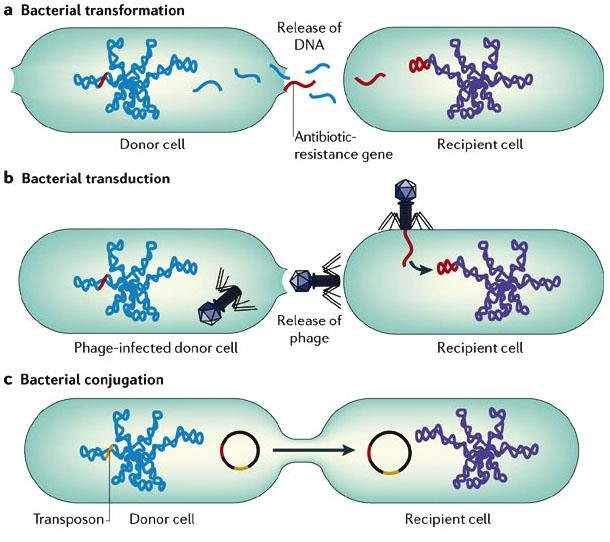
\includegraphics[width=0.5\textwidth]{figures/HGTExample.png}
		\caption{Biological mechanisms underlying horizontal gene transfer (HGT).\\From \href{https://www.researchgate.net/figure/Schematic-of-three-process-of-Horizontal-Gene-Transfer_fig2_277076640}{\textit{Nature Microbiology, © 2006  Nature Publishing Group}}}
		\label{fig:hgt-example}
	\end{figure}
	\\This can create cases where a gene in one species is unusually similar to a gene in a phylogenetically distant species. However, high similarity across distant taxa is not unique to HGT; such patterns may also result from strong functional conservation, heterogeneous evolutionary rates, gene loss in intermediate lineages, or annotation and assembly artifacts\cite{Dilucca2018}.
	Previous studies have identified numerous cases of HGT involving protein-coding genes in bacteria, most notably antibiotic resistance genes, such as the transmission of plasmids of $\beta$-lactamases \cite{Wang2023ISME} and rplB \cite{ManoharanBasil2021}. In addition, transfer of virulence factors, toxins, and genes involved in stress response and metabolism is also prevalent \cite{Soucy2015}. All these give the recipient organism a critical advantage in stressful environments.\\ \\
	Detecting HGT remains computationally challenging. Many established approaches either rely on phylogenetic incongruence (comparing gene trees to species trees), which is computationally heavy and sensitive to alignment quality, or use simpler heuristics (e.g., best-hit similarity, composition statistics) that are potentially over-simplified and noisy \cite{MishraLercher2025}.\\
	Our project explores a complementary, lightweight approach: represent cross-species gene similarities as a \textcolor{red}{sparse?} graph and use global graph patterns (together with species-distance context) to prioritize candidate HGT genes.
	
	\subsection{Research Question}
	How can graph-based analysis of gene similarity reveal candidate horizontal gene transfer events across bacterial genomes?
	
	\subsection{Hypothesis}
	We hypothesize that genes involved in horizontal gene transfer will exhibit disproportionately high similarity to phylogenetically distant species relative to background similarity patterns, forming graph edges that deviate from expected species-level clustering.
	
	\subsection{Objectives}
	\begin{itemize}[noitemsep, topsep=0pt]
		\item Construct a sparse gene similarity graph across multiple bacterial species using protein sequences
		\item Partition proteins into homologous groups using sequence-based clustering and construct within-group similarity graphs
		\item Define and compute an anomaly score that highlights unusually high similarity across large phylogenetic distances
		\item Generate interpretable visualizations (e.g., candidate ego-graphs)
		\item Validate high-scoring candidates by cross-referencing known functional annotations and reported HGT-related genes in the literature
	\end{itemize}
	
	\section{Data}
	\label{sec:data}
	As detailed below, our project was split into 2 methodologies. Both methodologies used data from NCBI RefSeq \cite{RefSeq}, and the NCBI Taxonomy database \cite{NCBITaxonomy} (using \texttt{BioPython}'s \texttt{Entrez} module \cite{BioPythonEntrez}).
	For each genome, we have FASTA files (\texttt{.faa}), where each entry corresponds to a single gene.\\
	Both methodologies used different data from RefSeq, due to a lack of coordination. \\
	For \hyperref[subsec:method1]{the first methodology}, we downloaded the \texttt{bacteria.*.protein.faa.gz} files from the bacteria database \cite{RefSeqBacteria}, which consist of 15 bacterial proteomes.\\
	For \hyperref[subsec:method2]{the second methodology}, we used a script to download protein sequences of 48 species spanning 19 families (e.g. gut microbiota, human pathogens) from the genome database \cite{RefSeqGenome}, \textcolor{red}{aimed to maximize detection of HGT events across phylogenetically diverse families}. The script \texttt{refseq\_fetch\_proteins.py} is available \href{https://github.com/noam-kimhi/Who-Stole-My-Genes/blob/main/Method\%202/src/graph_construction/refseq_fetch_proteins.py}{in the GitHub repository}. To control dataset size, we selected up to two assemblies per species using a deterministic
	ranking. While this choice ensured manageable scale and consistent annotation quality, it introduced some redundancy due to near-identical assemblies; we discuss this limitation in \textcolor{red}{add ref to discussions}.
	
	\section{Methods}
	Our work was split into 2 methodologies, both aimed to find HGT candidates using graph-based analysis, but from different perspectives. \hyperref[subsec:method1]{The first method} focused at the protein level, and \hyperref[subsec:method2]{the second} at the proteome level. Instead of using MSA and computationally intensive similarity calculations on entire proteomes, our methods employ the “divide and conquer” approach, each in its own way, in order to ease the computation.
	
	\subsection{Method 1 -- Identifying HGT Candidates Using Orthologous Clustering}
	\label{subsec:method1}
	This method seeks to locate similarly functional genes (orthologs) using sequence similarity clustering, and analyze each orthogonal group separately.
	The underlying assumption is that genes involved in HGT will cluster with functionally similar sequences across species, reducing the need for excessive similarity computations. This method consists of four main steps, as described in \cref{fig:method1-workflow}.
	\begin{figure}[htbp]
		\centering
		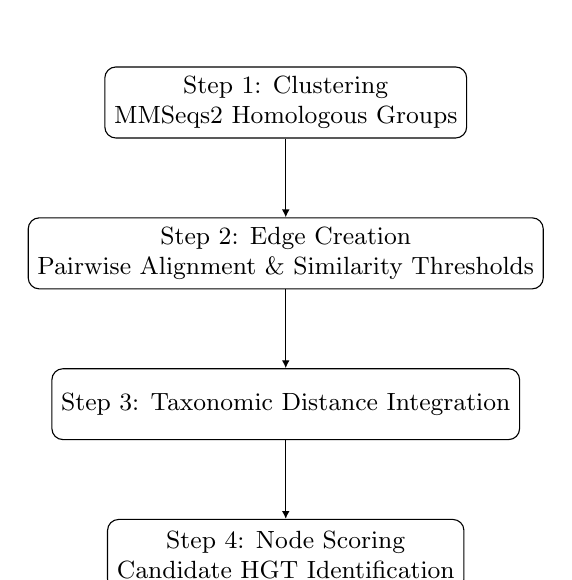
\begin{tikzpicture}[
			node distance=1cm,
			every node/.style={font=\small},
			box/.style={
				rectangle, draw, rounded corners,
				align=center, minimum width=4.5cm, minimum height=0.9cm
			},
			arrow/.style={
				-{Latex[length=1mm,width=1mm]},
				line width=0.5pt
			}
			]
			
			\node[box] (step1) {Step 1: Clustering \\ MMSeqs2 Homologous Groups};
			\node[box, below=of step1] (step2) {Step 2: Edge Creation \\ Pairwise Alignment \& Similarity Thresholds};
			\node[box, below=of step2] (step3) {Step 3: Taxonomic Distance Integration};
			\node[box, below=of step3] (step4) {Step 4: Node Scoring \\ Candidate HGT Identification};
			
			\draw[arrow] (step1) -- (step2);
			\draw[arrow] (step2) -- (step3);
			\draw[arrow] (step3) -- (step4);
			
		\end{tikzpicture}
		
		\caption{Workflow of \hyperref[subsec:method1]{Method 1}. Proteins are first clustered into homologous groups, followed by within-cluster alignment to construct similarity edges. Taxonomic distance is incorporated to detect anomalous cross-species similarities, and node-level scoring is used to identify candidate HGT genes.}
		\label{fig:method1-workflow}
	\end{figure}
	
	\subsubsection{Clustering}
	As discussed in \hyperref[sec:data]{the data section}, we downloaded protein sequences of 15 bactrial proteomes. We then clustered all proteins into homologous groups using MMseqs2 \cite{Steinegger2017MMseqs2}. We used a minimum sequence identity threshold of 50\% and a coverage threshold of 80\% (MMseqs2 parameters: \texttt{--min-seq-id 0.5} \texttt{-c 0.8}), so that sequences grouped together are broadly similar and likely to share related function.
	This clustering step constitutes the “divide” stage of our divide-and-conquer approach: downstream similarity computations are restricted to within-cluster comparisons, avoiding exhaustive comparisons across the full set of proteins.
	
	\subsubsection[Step 2]{Edge Creation Based on Similarity Score}
	\label{subsubsec:step2}
	Within each homologous cluster, we computed pairwise sequence alignments between all unordered protein pairs. Alignments were performed using the \texttt{PairwiseAligner} class from \texttt{Biopython} (v1.85), configured for local alignment (mode \texttt{local}) with the BLOSUM62 substitution matrix \cite{BLOSUM}. Gap penalties were set to a gap opening score of $-10$ and a gap extension score of $-1$.
	For each aligned pair $(u,v)$, we computed the following metrics:
	\[
	\text{Identity}(u,v) =
	\frac{\#\text{matching aligned residues}}
	{\min\{\text{len}(u), \text{len}(v)\}}
	\]
	
	\[
	\text{Coverage}(u,v) =
	\frac{\text{aligned\_length}}
	{\min\{\text{len}(u), \text{len}(v)\}}
	\]
	An undirected edge between $u$ and $v$ was created only if:
	\begin{center}
		$\text{Identity} \ge 0.5$, \quad
		$\text{Coverage} \ge 0.8$, \quad
		$\text{aligned\_length} \ge 50$
	\end{center}
	The minimum aligned length of 50 residues was chosen to avoid spurious edges arising from short conserved motifs or domain fragments. For each edge, we defined the similarity score as:
	\begin{center}
		$\text{SimilarityScore}(u,v) = \text{Identity}(u,v) \times \text{Coverage}(u,v).$
	\end{center}
	For a cluster containing $n$ proteins, this procedure requires $O(n^2)$ pairwise alignments. Since clustering partitions the full dataset into smaller groups, $n$ is typically much smaller than the total number of proteins, making this computation feasible. For pseudo-code, see \cref{algo1}.
	\begin{algorithm}
		\caption{BuildEdgesFromAlignments}
		\begin{algorithmic}[1]
			\State \textbf{Input:} Dictionary $seqs$
			\State \textbf{Output:} List $edges$
			
			\State $ids \gets$ sorted keys of $seqs$
			\State $edges \gets \emptyset$
			
			\ForAll{unordered pairs $(u,v)$ in $ids$}
			\State $(identity, coverage, aligned\_len) \gets$ align($seqs[u], seqs[v]$)
			
			\If{$identity \ge 0.5$ \textbf{and} $coverage \ge 0.8$ \textbf{and} $aligned\_len \ge 50$}
			\State $score \gets identity \times coverage$
			\State Add edge $(u,v)$ with attributes $(score, identity, coverage, aligned\_len)$ to $edges$
			\EndIf
			\EndFor
			
			\State \Return $edges$
		\end{algorithmic}
		\label{algo1}
	\end{algorithm}
	
	\subsubsection[Step 3]{Incorporating Taxonomic Information and Computing Distance}
	\label{subsubsec:step3}
	To contextualize cross-species similarities, we retrieved taxonomic lineage information for each species represented in the graph using the NCBI Taxonomy database \cite{NCBITaxonomy}.
	Each graph node was annotated with taxonomic attributes corresponding to the ordered rank list:
	\begin{center}
		(\text{species}, \text{genus}, \text{family}, \text{order}, \text{class}, \text{phylum}, \text{superkingdom})
	\end{center}
	For two species $u$ and $v$, we define their taxonomic distance based on the most specific (lowest) rank at which they share the same annotation.  
	Formally, let the ordered rank list be indexed from $0$ (species) to $\mathcal{R}-1$ (superkingdom).  
	The taxonomic distance $d(u,v)$ is defined as:
	{\setlength{\abovedisplayskip}{4pt}
		\setlength{\belowdisplayskip}{4pt}
		\begin{equation*}
			d(u,v) = \min\left\{ i \mid \text{$u$ and $v$ share the same label at rank } i \right\}
		\end{equation*}
	}
	If the two species do not share any common annotation across the considered ranks, we set $d(u,v) = \mathcal{R}$. Thus, smaller values of $d(u,v)$ indicate closer phylogenetic relatedness, while larger values correspond to more distant taxa.
	
	\subsubsection[Step 4]{Node Scoring and Identification of HGT Candidates}
	\label{subsubsec:step4}
	We flagged an edge $(u,v)$ as suspicious if it simultaneously connected distant taxa and highly similar proteins:
	\begin{center}
		$d_{\text{tax}}(u,v) \ge 2
		\quad\textbf{and}\quad
		\mathrm{SimilarityScore}(u,v) \ge 0.6$
	\end{center}
	where $d_{\text{tax}}(u,v)$ is the taxonomic distance from \nameref{subsubsec:step3}, and $\mathrm{SimilarityScore}$ is defined in \nameref{subsubsec:step2}.
	Intuitively, such edges represent unexpected cross-species similarity (large taxonomic distance, yet high sequence similarity).\\
	Let $S(i)$ denote the set of nodes connected to $i$ by suspicious edges.
	We then compute two quantities for every node $i$:
	\begin{enumerate}[noitemsep]
		\item \textbf{HGT score} (sum of similarity scores over suspicious edges):
		{\setlength{\abovedisplayskip}{4pt}
			\setlength{\belowdisplayskip}{4pt}
			\begin{equation*}
				\mathrm{score}(i) = \sum_{j \in S(i)} \mathrm{SimilarityScore}(i,j)
			\end{equation*}
		}
		\item \textbf{Suspicious degree} (number of suspicious edges incident to $i$):
		{\setlength{\abovedisplayskip}{4pt}
			\setlength{\belowdisplayskip}{4pt}
			\begin{equation*}
				\deg_{\text{sus}}(i) = |S(i)|
			\end{equation*}
		}
	\end{enumerate}
	To select candidate HGT proteins, we considered only nodes with $\deg_{\text{sus}}(i)\ge 2$ and whose score exceeded a threshold that we needed to determine.
	We found the $70$th percentile of the non-zero node scores (denoted as $\tau_{\text{score}}$) and retained nodes satisfying 
	\begin{center}
		$\mathrm{score}(i)\ge \tau_{\text{score}}
		\quad\textbf{and}\quad
		\deg_{\text{sus}}(i)\ge 2$
	\end{center}
	We ranked candidates by score and reported the top-ranked node(s). In our experiments we output the top 1 candidate(\texttt{TOP\_HGT\_N}$=1$). i.e. the node with the highest HGT score, which also could (but not necessarily) be the gene donor. \\
	Finally, we supported the top candidate using phylogenetic reconstruction.
	Phylogenetic trees were constructed with the Neighbor-Joining (NJ) algorithm \cite{NJ} using the pairwise distance:
	\[
	d(u,v)=1-\mathrm{Identity}(u,v),
	\]
	where $\mathrm{Identity}(u,v)$ is computed as in \nameref{subsubsec:step2}. If a pairwise identity was unavailable, we set $d(u,v)=1$.
	
	\subsection{Method 2 -- Alignment-Free Detection of HGT Candidates}
	\label{subsec:method2}
	An overview of the pipeline is shown in \cref{fig:pipeline_overview}.
	
	\begin{figure}[h]
		\centering
		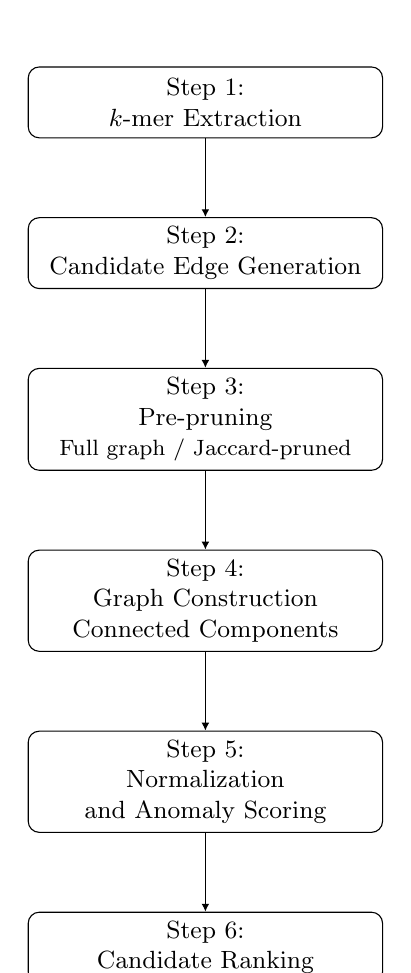
\begin{tikzpicture}[
			node distance=1cm,
			every node/.style={font=\small},
			box/.style={
				rectangle, draw, rounded corners,
				align=center, minimum width=4.5cm, minimum height=0.9cm
			},
			arrow/.style={
				-{Latex[length=1mm,width=1mm]},
				line width=0.5pt
			}
			]
			
			\node[box] (kmers) {Step 1: \\ $k$-mer Extraction};
			\node[box, below=of kmers] (cand) {Step 2: \\ Candidate Edge Generation};
			\node[box, below=of cand] (prune) {Step 3: \\ Pre-pruning\\{\footnotesize Full graph / Jaccard-pruned}};
			\node[box, below=of prune] (graph) {Step 4: \\ Graph Construction\\Connected Components};
			\node[box, below=of graph] (score) {Step 5: \\ Normalization\\and Anomaly Scoring};
			\node[box, below=of score] (rank) {Step 6: \\ Candidate Ranking};
			
			\draw[arrow] (kmers) -- (cand);
			\draw[arrow] (cand) -- (prune);
			\draw[arrow] (prune) -- (graph);
			\draw[arrow] (graph) -- (score);
			\draw[arrow] (score) -- (rank);
		\end{tikzpicture}
		\caption{Workflow of \hyperref[subsec:method2]{Method 2}. Protein sequences are represented using $k$-mers to
			generate cross-species similarity candidates. Pre-pruning controls graph density by retaining high-confidence
			edges, after which normalization and graph-based anomaly scoring are applied to identify candidate
			HGT-related proteins.}
		\label{fig:pipeline_overview}
	\end{figure}
	
	\subsubsection{Similarity Candidate Generation}
	To avoid computationally infeasible all-vs-all alignments, proteins shorter than 50 amino acids were excluded. The remaining sequences were represented as sets of distinct $k$-mers ($k=6$), encoded as collision-free base-20 integers over the canonical amino acid alphabet\cite{Sims2009,Haubold2014}.\\
	To suppress non-informative overlaps, highly frequent $k$-mers (posting list size $>100$) were excluded. Only cross-species pairs were considered, as intra-species similarity is expected and not informative for HGT detection, and candidate lists were capped to the top 10 matches per protein. Exact Jaccard similarity over the $k$-mer sets was then computed for these candidate pairs to obtain deterministic similarity scores.
	
	\subsubsection{Graph Construction and Pruning}
	Candidate pairs were assembled into an undirected, weighted similarity graph, with edges weighted by Jaccard similarity of $k$-mer sets. Similarities were normalized per species pair by retaining the strongest edges (top 10\% per pair). All retained edges were required to meet a minimum Jaccard similarity value of 0.1, and per-node degree was capped at 20.\\	
	Additional taxonomic distance filters retained edges with taxonomic distance in the range $[2,4]$, that was calculated as shown in \hyperref[subsec:method1]{Method 1}'s \nameref{subsubsec:step3}. These steps reduced the graph from approximately $9\times 10^5$ candidate edges to 92,790 edges, yielding the sparse graph used to detect HGT events.
	
	\subsubsection{Graph-Based Anomaly Scoring}
	Graph structure enables evaluation of anomalous similarity within mixed-species components. Similarity scores were normalized using robust $z$-scores based on the median and MAD\cite{Rousseeuw1993}, and were computed per species pair when more than 30 edges were available.\\
	Within each connected component of the pruned graph, taxonomic mixing was quantified using species count and normalized Shannon entropy \cite{ShannonEntropy}. Anomaly concentration was measured as the fraction of edges with $z\ge3$. Each node was annotated with anomaly evidence (max and top-k mean $z$-scores) and structural connectivity metrics: cross-species degree, neighbor entropy, participation coefficient\cite{Guimera2005}, clustering coefficient, and betweenness centrality.\\
	Proteins were ranked using a scoring framework with threshold gates requiring sufficient component size, taxonomic mixing, anomalous similarity, and cross-species connectivity (component size $\ge10$, entropy $\ge0.75$, node degree $\ge4$, mean top-5 $z\ge2$).
	
	\begin{equation}
		\log S(u) = \log \Phi(C_u) + \log A(u) + \log T(u),
	\end{equation}
	
	$\Phi(C_u)$ captures component-level taxonomic mixing and anomaly concentration, $A(u)$ aggregates normalized similarity scores, and $T(u)$ summarizes cross-species connectivity and bridge-like topology. To stabilize scale differences across components, aggregation was performed in log-space, meaning high scores arise only when anomaly and structural evidence co-occur.
	
	\section{Results}
	\subsection{Constructed Graph}
	In \hyperref[subsec:method2]{method 2}, we created a candidate graph which can be used to find HGT events.\\
	The full candidate graph contains 911,306 cross-species edges over 214,136 proteins. After Jaccard-based pre-pruning it contains 92,790 edges over 37,421 proteins across 5,262 connected components.\\
	Component size is highly skewed (median 4; 95th percentile 20; max 107). Median components span two species, and only 18.5\% contain more than 5 species.\\
	Anomalous similarity is globally sparse: the median fraction of high-$z$ edges per component is 0 and only 3.9\% of components show substantial anomaly concentration ($high\_z\_frac >0.3$). This sparsity is also evident in the global edge distribution (\cref{fig:zscoredist}), where most similarities cluster near the baseline while high-$z$ edges occupy a small right tail.\\	
	Across 37,421 proteins in the pruned graph, only 5.9\% satisfy the gating criteria and receive a non-zero score, indicating strong selectivity.
	
	\subsection{Findings}
	The methodologies we developed are designed to show candidates to HGT genes. After finding those, we needed to biologically validate them to prove they are in fact valid candidates for HGT events. We will now present some of the candidates, along with biological background to support the findings.
	
	\subsubsection{Horizontal Transfer of EptC (Phosphoethanolamine Transferase)}
	Using \hyperref[subsec:method1]{method 1}, we identified EptC as a candidate HGT event. EptC is an enzyme that catalyzes the addition of a phosphoethanolamine (PEA) group to components of the bacterial outer membrane. This modification reduces the net negative charge of the membrane surface. Antimicrobial peptides produced by the host are predominantly positively charged. By decreasing the membrane’s negative charge, the enzyme discourages the entrance of antimicrobial peptides and mitigtes their immunological effect. This provides a selective advantage to the bacterium. EptC is a known HGT-associated gene \cite{Zinkle2025}.\\
	In \cref{fig:EptC_graph} below we show a similarity graph in which a red thick line is connecting \textit{Shigella} to two \textit{Escherichia Coli} species.
	In addition to the thick lines between \textit{Shigella} and \textit{E. coli}, we observe low similarity between \textit{Pseudomonas Aeruginosa} (cyan node) and the other bacteria, suggesting our results are not due to conservation, but rather an HGT event. Also note how there is no suspicious edge between the two strains of \textit{E. coli}, thanks to integration of taxonomic information in our suspects filtering. \\
	\begin{figure}[H]
		\centering
		\includegraphics[width=0.5\textwidth]{figures/EptC_graph.png}
		\caption{Similarity graph for the EptC gene. Each node denotes a protein and the text above denotes the origin species. The thicker the edge, the higher the similarity score between the proteins, A red edge hints at a potential HGT event.}
		\label{fig:EptC_graph}
	\end{figure}
	\noindent
	Then, we turned to construct a gene phylogenetic tree to see which species are closest. As mentioned in \nameref{subsubsec:step4}, trees were constructed using the NJ algorithm \cite{NJ}. As expected from HGT, we got close relations between one strain of \textit{E. coli}, \textit{Shigella}, and \textit{Salmonella}, differing from the species tree, which would join the two \textit{E. coli} strains to each other.
	\begin{figure}[H]
		\centering
		\includegraphics[width=0.7\textwidth]{figures/EptC_tree.png}
		\caption{Constructed phylogenetic tree for the EptC coding gene. Note the abnormal distance between \textit{E. coli} strains, suggesting HGT event.}
		\label{fig:EptC_tree}
	\end{figure}
	
	\subsubsection{Horizontal Transfer of ymdF}
	Using the \hyperref[subsec:method1]{method 1}, we identified ymdF as an additional candidate HGT event. At the time of writing this report, the exact function of the protein itself remains a mystery to the scientific community, although it is annotated as a stress-induced or stress-related protein \cite{Keseler2017EcoCyc, BioCyc_G0-10443}. Proteins involved in stress response can confer a selective advantage under adverse conditions, making such genes plausible candidates for horizontal acquisition. While there is no direct HGT evidence of ymdF itself, it has been proposed that the yciFE operon, which includes paralogs of ymdF, comprises horizontally transferred genes in both \textit{E. coli} and \textit{Salmonella} \cite{Oguri2018}, suggesting an HGT history of related genes within this operon. HGT is further supported again by our phylogenetic analysis.
	In \cref{fig:ymdF_graph}, we present the similarity graph for the ymdF protein constructed using \hyperref[subsec:method1]{method 1}. As previously reported, the yciFE operon, which contains paralogs of ymdF, has been shown to be closely related between \textit{E. coli} and \textit{Salmonella} \cite{Oguri2018}. This relationship is clearly recovered by our graph, as indicated by the thick red edge connecting the corresponding nodes (purple and brown). Note that one node (gray) lacks species annotation in our dataset.\\
	\begin{figure}[hbtp]
		\centering
		\includegraphics[width=0.7\textwidth]{figures/ymdF_graph.png}
		\caption{Similarity graph for the ymdF protein. The thicker the edge, the higher the similarity score between the proteins. A red edge hints at a potential HGT event.}
		\label{fig:ymdF_graph}
	\end{figure}
	\noindent
	In \cref{fig:ymdF_tree} we see the gene tree of ymdF. The tree suggests a close similarity between an \textit{E. coli} strain and \textit{Salmonella}, instead of the expected similarity between the two \textit{E. coli} strains, supporting the clain of an HGT event.
	\begin{figure}[hbtp]
		\centering
		\includegraphics[width=0.7\textwidth]{figures/ymdF_tree.png}
		\caption{Constructed phylogenetic tree for the ymdF coding gene. Note the abnormal distance between \textit{E. coli} strains, suggesting HGT event.}
		\label{fig:ymdF_tree}
	\end{figure}
	
	\FloatBarrier
	
	\subsubsection{Structural regimes in the Jaccard-pruned graph}
	
	\begin{table}[t]
		\centering
		\small
		\begin{tabular}{lrrrrrr}
			\toprule
			Component & Proteins & Edges & Density & Species & $H_{\mathrm{norm}}$ & high-$z$ frac \\
			\midrule
			5  & 97 & 632 & 0.136 & 50 & 0.998 & 0.60 \\
			8  & 95 & 589 & 0.130 & 49 & 0.998 & 0.47 \\
			32 & 71 & 332 & 0.134 & 31 & 0.958 & 0.063 \\
			\bottomrule
		\end{tabular}
		\caption{Summary statistics for representative components in the pruned similarity graph.}
		\label{tab:components}
	\end{table}
	
	\begin{figure}[!t]
		\centering
		\includegraphics[height=0.45\textheight]{figures/component_5.png}
		\caption{Component 5: Broad multi-taxa exchange module. Nodes represent proteins and edges represent cross-species similarity. Node size reflects candidate score, and highlighted edges correspond to high-surprise similarities relative to species-pair baselines.}
		\label{fig:component5}
	\end{figure}
	
	\begin{figure}[!t]
		\centering
		\includegraphics[height=0.45\textheight]{figures/component_8.png}
		\caption{Component 8: Chained cross-species connectivity. Compact sub-clusters are linked by a small number of high-surprise edges, producing elongated paths across distant taxa.}
		\label{fig:component8}
	\end{figure}
	
	\begin{figure}[t]
		\centering
		\includegraphics[width=\linewidth]{figures/component_32.png}
		\caption{Component 32: Localized high-confidence bridges. Two coherent regions are connected by a small number of strong cross-species edges, with anomalous signal concentrated in the bridges.}
		\label{fig:component32}
	\end{figure}
	
	Three representative components illustrate distinct structural regimes of cross-species similarity (\cref{tab:components}).
	Component 5 forms a dense multi-taxa exchange module spanning many species with near-maximal entropy and strong anomaly concentration (\cref{tab:components}, \cref{fig:component5}). High-scoring proteins participate in multiple cross-species interactions, suggesting a shared exchange module rather than isolated anomalies.
	
	Clusters within this component correspond to horizontally transferred ribosomal proteins. 
	The left cluster involves ribosomal protein S21, which has been linked to late-stage phage replication and can become part of the phage genetic toolkit used to hijack host translational machinery after transfer \cite{phage_S21_hgt,frontiers_hgt_tools}. 
	In contrast, the top and right clusters correspond to ribosomal protein S12 (encoded by \textit{rpsL}) within the 30S ribosomal subunit, whose mutations are associated with streptomycin resistance \cite{rpsL_streptomycin}.
	
	Component 8 shows a chained transfer-like topology spanning many taxa with high entropy and substantial anomaly concentration (\cref{tab:components}, \cref{fig:component8}). Compact subclusters are linked by a few high-surprise edges, producing elongated paths consistent with stepwise propagation across lineages. 
	
	Clusters in this component correspond to horizontal transfer of the 30S ribosomal protein S10 (encoded by \textit{rpsJ}), whose mutations are known markers of tigecycline resistance\cite{rpsJ_tigecycline}. Horizontal transfer of this gene has been reported among \textit{Mycobacterium} species, including \textit{M. tuberculosis} \cite{mycobacterium_rpsJ_transfer}.
	
	Component 32 instead exhibits localized high-confidence bridges across many species but with relatively low anomaly concentration (Table~\ref{tab:components}, Figure~\ref{fig:component32}). Here anomalous signal concentrates in a few bridging edges linking otherwise ordinary similarity neighborhoods. 
	
	Clusters in this component correspond to horizontal transfer of glucose-1-phosphate thymidylyltransferase, a key enzyme in bacterial surface polysaccharide biosynthesis. Such polysaccharides contribute to host immune evasion; for example, Capnocytophaga (pathogenic oral commensal in dogs) species use them to resist the bactericidal effects of human serum\cite{capnocytophaga_surface_polysaccharide,capnocytophaga_serum_resistance}.
	
	\subsubsection{Comparison with the full candidate graph}
	
	Applying the same normalization and structural scoring to the full candidate graph yields substantially denser connectivity, with many additional proteins and edges that obscure component boundaries. This contrast supports pre-pruning as a practical requirement for interpreting anomalous similarity patterns at scale.
	
	\subsubsection{Score distribution and selectivity}
	
	Among the top 200 ranked proteins, the median score was 5.9 (IQR: 4.47–8.17), with the 95th percentile at 12.74 and a maximum of 18.76. These values represent the extreme upper tail of the scoring distribution among the 5.9\% of proteins that passed gating.
	
	\FloatBarrier
	\section{Discussion}
	\textcolor{red}{\uline{\textbf{Method 2 - Sketching approaches such as MinHash could further scale the pipeline to larger datasets\cite{Broder1997,Ondov2016}.}}}
	
	
	\newpage
	
	\bibliographystyle{unsrturl}
	\bibliography{references}
	
	
\end{document}
